\documentclass[aspectratio=169,12pt]{beamer}
%\documentclass[handout]{beamer}

% ### Preamble

% Encoding
\usepackage[utf8]{inputenc} % Use utf8 encoding in the input (.tex) file
\usepackage[english]{babel} % Load characters and hyphenation
\usepackage[T1]{fontenc} % Use utf8 encoding in the output (.pdf) file
\usepackage[english=british]{csquotes} % Quote like a boss

% Decorations
\usepackage{microtype} % Improves character and word spacing
\usepackage{booktabs} % Better horizontal rules in tables
\usepackage{multicol} % Customisation for tables
\usepackage{amsmath} % Improved mathematics

% Debug: grids
%\setbeamertemplate{background}[grid][step=1mm]

% Size
% With an aspect ratio of 16:9, I prefer having wide margins
\setbeamersize{text margin left=1.4cm}
\setbeamersize{text margin right=1.4cm}

% Presentation structure
\usepackage{appendixnumberbeamer} % Allows for an appendix

% Special content
\usepackage{textgreek} % Greek characters
\usepackage{units} % Used for printing standard units
\usepackage[scale=2]{ccicons} % Creative Commons icons

% Bibliography
\usepackage[sortcites,citestyle=verbose,backend=biber]{biblatex} 
\addbibresource{../main.bib}
\AtEveryBibitem{%
	\clearfield{url}%
	\clearfield{issn}%
	\clearfield{isbn}%
	\clearfield{archivePrefix}%
	\clearfield{arxivId}%
	\clearfield{pmid}%
	\clearfield{eprint}%
	\clearfield{doi}%
	\clearfield{number}%
	\clearfield{pages}%
	\clearfield{volume}%
}
% https://tex.stackexchange.com/questions/25891/fullcite-without-indent-in-biblatex
\AtEveryCitekey{%
	\clearfield{issn}%
	\clearfield{url}%
	\clearfield{archivePrefix}%
	\clearfield{arxivId}%
	\clearfield{eprint}%
}

% Images
\usepackage{graphicx}
\graphicspath{ {../images/} }
\setkeys{Gin}{keepaspectratio} % Improves figure scaling
\setlength\abovecaptionskip{+5pt}
\usepackage{caption}
\captionsetup{font=footnotesize}

% Themes, colours and fonts
% Choose the theme according to the purpose of the presentation; do not 
% become too attached to a particular theme. For long presentations, a 
% sidebar which highlights the current topic can be helpful.
% Themes
\usetheme[
	progressbar=frametitle,
	%progressbar=foot,
	numbering=fraction,
	%sectionpage=simple,
	block=fill,
]{metropolis} % A modern theme
%\usetheme{Madrid} % A classic
%\usetheme{Hannover} % Side bar
% Colour themes
%\usecolortheme{seagull} % Gray-based
%\usecolortheme{crane} % Straw yellow
% Fonts
\usepackage{FiraSans} % Font needed by metropolis
\usepackage{FiraMono} % Font needed by metropolis
\usepackage{amsfonts} % Math fonts
\usepackage{xspace} % Print a space better than a ~

\newcommand{\etal}{\textit{et al.}\xspace}

%\definecolor{mLightBrown}{HTML}{EB811B}
%\newcommand{\alert}[1]{\textcolor{mLightBrown}{#1}} % Print text in 
%orange

% Table of contents
%\setbeamertemplate{section in toc}[sections numbered] % ToC style
%\AtBeginSection[] % Recurring ToC
%{
%	\begin{frame}
%		\frametitle{Table of Contents}
%    	\tableofcontents[currentsection]
%	\end{frame}
%}

% Footer
% Remember: if everyone in the audience knows you, putting your name at 
% the bottom of each slide is just vanity.
%\setbeamertemplate{frame footer}{\tiny Footer} 

% Notes and printing layout settings

\usepackage{pgfpages} % Manage page layout 
%\pgfpagesuselayout{4 on 1}[a4paper,border shrink=0mm,landscape]
%\setbeameroption{show notes} % Print note after corresponding frame
%\setbeameroption{show only notes} % Print only notes
%\setbeameroption{show notes on second screen} % (Self explainatory)
\setbeamertemplate{note page}[plain] % Use minimal notes
\AtBeginNote{\scriptsize}

% Insert a subtitle in the section page
% Thanks to 
% https://tex.stackexchange.com/questions/404224/beamer-metropolis-theme-add-image-to-section-page
\makeatletter
\defbeamertemplate*{section page}{mytheme}[1][]{
  \centering
  \begin{minipage}{25em}
    \raggedright
    \usebeamercolor[fg]{section title}
    \usebeamerfont{section title}
    \insertsectionhead\\[-1ex]
    \usebeamertemplate*{progress bar in section page}
    \par
    \ifx\insertsubsectionhead\@empty\else%
      \usebeamercolor[fg]{subsection title}%
      \usebeamerfont{subsection title}%
      \insertsubsectionhead
    \fi
    \vskip0.5cm
    \ifstrempty{#1}{}{%
		\centering%
		\footnotesize #1%
    }
  \end{minipage}
  \par
  \vspace{\baselineskip}
}
\makeatother

\newcommand{\sectionquote}[2]{
	\setbeamertemplate{section page}[mytheme][#2]
	\section{#1}
	\setbeamertemplate{sectionpage}[mytheme]
	% Revert the changes to the section page
	\metroset{sectionpage=progressbar}
}

% ### Top matter

\title{Transcriptome-Wide Association Studies}
\subtitle{\normalsize Bridging the gap between genome, transcriptome and 
disease}
\author[Federico Marotta]
{
	\footnotesize
	Supervisor: \href{mailto:paolo.provero@unito.it}{Prof. Paolo 
		Provero}
	\\
	Candidate: \href{mailto:federico.marotta@edu.unito.it}{Federico 
		Marotta}
	\vfill
	\scriptsize
	Università degli Studi di Torino
	\\
	Dipartimento di Biotecnologie Molecolari e Scienze per la Salute
	\vfill
}
\institute[UniTo, DBMSS]
{
	%\scriptsize
	%\bigskip

	%Università degli Studi di Torino\\
	%Dipartimento di Biotecnologie Molecolari e Scienze per la Salute

	%\bigskip
	%\vfill

	%{\tiny {\ccbysa\/}
	%\href{https://creativecommons.org/licenses/by-sa/4.0/}
	%{CC BY-SA}}
}
%\date{\tiny Tesi di Laurea, 18\textsuperscript{th} July 2018}
\date{\tiny Tesi di Laurea, 18 luglio 2018}

% ### Document

\begin{document}

\maketitle

% Table of contents
% It can seem silly in a ten-minute presentation.
% NOTE: This frame is mutually exclusive with a recurring ToC.
%\begin{frame}
	%\frametitle{Outline}
	%\tableofcontents
%\end{frame}

\begin{frame}{Nature or Nurture: that is the question}

	\bigskip

	\begin{block}{Complex diseases:}
		As opposed to Mendelian diseases, complex ones cannot be 
explained by a mutation in a single gene
	\end{block}

	\bigskip

	Do they have a genetic basis at all?

	\pause

	\begin{itemize}
		\item Initially, there were \alert{linkage studies} and 
			\alert{candidate-gene association studies}
		\item Gradually, the focus moved towards \alert{populations and 
				whole genomes}
		\item \alert{GWAS}, especially if combined with eQTL mapping and 
			functional annotations, have found many risk SNPs
	 \end{itemize}

	\note[item]{Interaction of many genes with each other and with the 
		environment}
	\note[item]{We have seen with Alessandro Lussana that non coding 
		variants are important}
	\note[item]{To answer the question, many methods were developed}
	\note[item]{A linkage study is... a candidate-gene association study 
		is... a GWAS is... eQTL mapping is...}
	\note[item]{Many SNP-disease association have been found}

\end{frame}

\begin{frame}{Gene expression, the missing link}

	\begin{figure}
		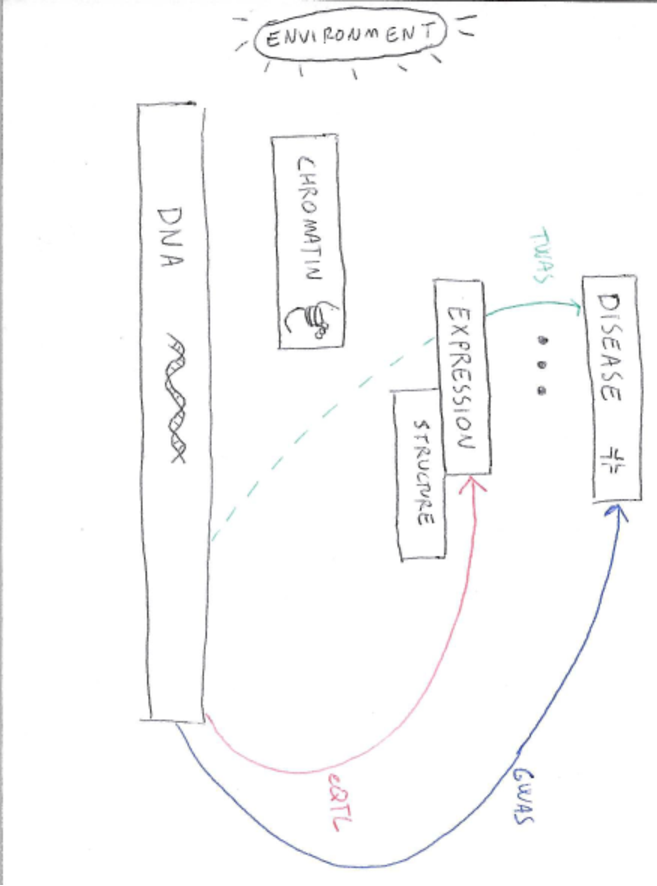
\includegraphics[width=0.9\textwidth]{introduction/summary}
		\caption{TWAS focus on the genetic component of expression}
	\end{figure}

\end{frame}

\sectionquote{A gene-based association method}{\cite{Gamazon2015}}

\begin{frame}{Training on reference transcriptome data sets}
	
	\begin{columns}
		\begin{column}{0.4\textwidth}
			The genetically regulated component of expression must be 
imputed

			\begin{equation*}
				T = w_1 X_1 + w_2 X_2 + \ldots
			\end{equation*}
		\end{column}

		\begin{column}{0.6\textwidth}
			\begin{figure}
				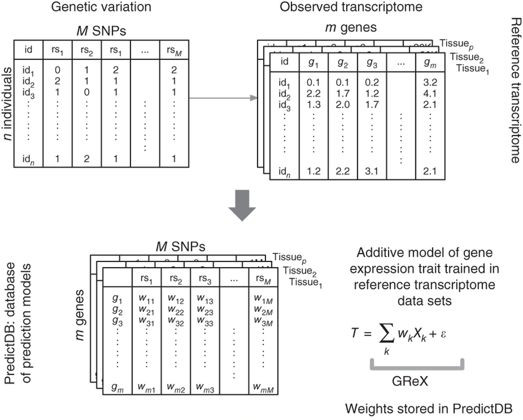
\includegraphics[width=\textwidth]{gamazon2015/2-grex_estimation_part1}
				\caption{Training of the SNP-expression model}
			\end{figure}
		\end{column}
	\end{columns}

	\note[item]{Phenotype-determined expression goes away because these 
are healthy individuals. The environment component goes away because it 
averages out in the regression model.}
	\note[item]{Even if we had expression data, we still would impute 
the GReX}

\end{frame}

\begin{frame}{Association of the imputed expression to the phenotype}
	
	\begin{figure}
		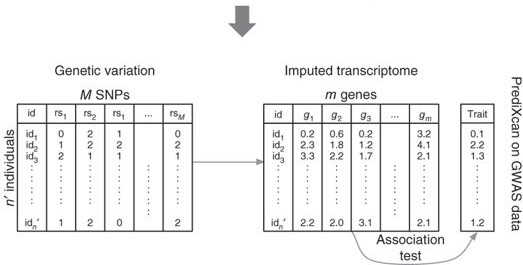
\includegraphics[width=0.8\textwidth]{gamazon2015/2-grex_estimation_part2}
		\caption{The actual TWAS}
	\end{figure}

	\note[item]{Logistic model. They could have modeled the liability to 
disease.}
	\note[item]{This is the real TWAS. The previous part was only needed 
because expression is not measured}

\end{frame}

\begin{frame}{Results in T1D}

	\begin{figure}
		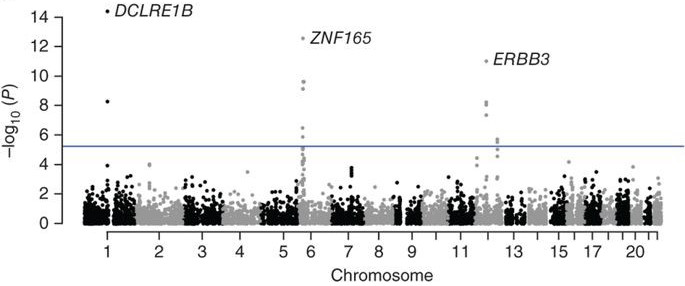
\includegraphics[width=0.9\textwidth]{gamazon2015/7-t1d_associations_manhattan}
		\caption{Manhattan plot of P-values for gene-disease 
associations}
	\end{figure}

	\note[item]{Why are nearby genes all associated? coregulation 
because of tad altered (upstream event)? This could be a pitfall of 
TWAS. See conclusions.}

\end{frame}

\sectionquote{Integrative approaches}{\cite{Gusev2016}}

\begin{frame}{From individual-level to summary-based TWAS}

	\begin{figure}
		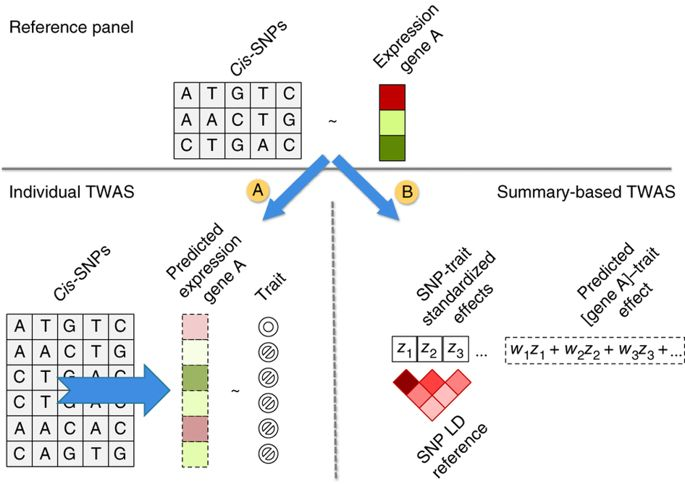
\includegraphics[width=0.8\textwidth]{gusev2016/1-TWAS_schematic}
	\end{figure}

	\note[item]{Individual-level data is not available}
	\note[item]{If a SNP is associated to a trait with score z_SNP, but 
it does not alter gene expression, its contribution to the association 
score of the gene to the trait is 0.}

\end{frame}

\begin{frame}{Application to obesity GWAS}

	The estimation of SNP weights was performed on \char`\~3000 
individuals

	\begin{itemize}
		\item When applied to a small-cohort GWAS, this approach found 
some genes that were only reported in a later large-cohort GWAS
	\end{itemize}

	\note[item]{First bullet: TWAS are more powerful. Indeed, less 
multiple testing.}

\end{frame}

\sectionquote{Moving beyond genetic variants alone}{\cite{Gusev2018}}

% NOTE: here the results will be more important. Previously we have 
% neglected them.

\begin{frame}{Integrating many types of data}

	\begin{columns}
		\begin{column}{0.6\textwidth}
			\begin{figure}
				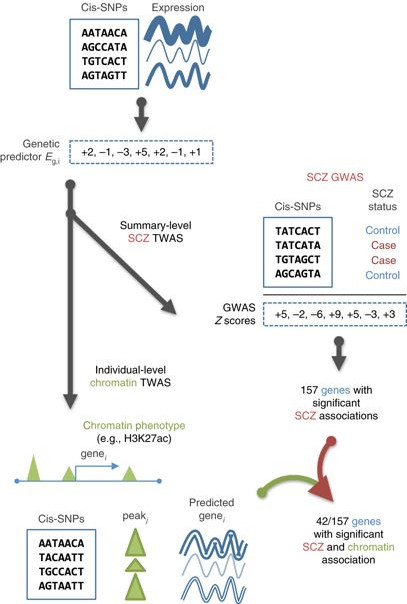
\includegraphics[width=0.62\textwidth]{gusev2018/1-TWAS_schematic_cropped}
			\end{figure}
		\end{column}

		\begin{column}{0.4\textwidth}
			\begin{itemize}
				\item Association does not imply mechanism
				\item Gene expression is not the only link
			\end{itemize}
		\end{column}
	\end{columns}

	\note[item]{Gene expression is one of the many intermediate 
phenotypes}

\end{frame}

\begin{frame}{A threefold pipe line}

	\begin{itemize}
		\item Schizophrenia TWAS
		\begin{itemize}
			\item 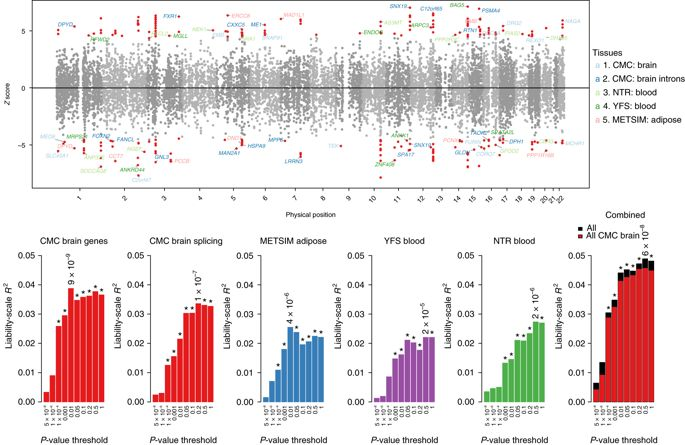
\includegraphics[width=0.7\textwidth]{gusev2018/2-schizophrenia_TWAS}
		\end{itemize}

		\item Chromatin TWAS
		\begin{itemize}
			\item Of the 157 SCZ-associated genes, 42 were also 
associated to a chromatin peak
		\end{itemize}

		\item Schizophrenia \enquote{Spliceome}-WAS
		\begin{itemize}
			\item 46 splicing events in the brain associated to disease
		\end{itemize}
	\end{itemize}

\end{frame}

\begin{frame}{Biological example: \textit{MAPK3}}
	
	\begin{itemize}
		\item \textit{MAPK3} and \textit{KCTD13} are coregulated
		\item \textit{KCTD13} decreases proliferation, \textit{MAPK3} is 
a functional trigger
	\end{itemize}

	\begin{figure}
		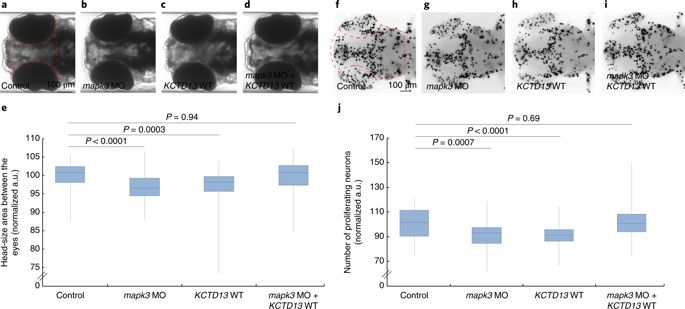
\includegraphics[width=0.8\textwidth]{gusev2018/6-zebrafish}
		\caption{Zebrafish over-expressing \textit{KCTD13}, with or 
without inhibition of \textit{MAPK3}}
	\end{figure}

	\note[item]{At last!}

\end{frame}

\begin{frame}{Conclusions}

	TWAS address some of the limitations of classical association 
studies:

	\begin{itemize}
		\item Increased interpretability and druggability
		\item No need to assemble large cohorts
	\end{itemize}

	But have limitations of their own:

	\begin{itemize}
		\item If expression is not involved, TWAS do not work
		\item Pleiotropy cannot be modeled
	\end{itemize}

\end{frame}

\begin{frame}{Future perspectives}

	\begin{itemize}
		\item<1-> An association study may be performed with any 
intermediate molecular phenotype
		\item<2-> And in any population
		\item<3-> Epistasis and dominance should be taken into account
		\item<4-> A \enquote{network approach} could help to further 
explain the results
	\end{itemize}

	\note[item]{Network approach: indeed in the last paper the 
association was with MAPK3, but the mechanism was explained by KCTD13}

\end{frame}

\appendix

\metroset{sectionpage=simple}

\begin{frame}[plain]
	\nocite{*}
	\tiny
	\printbibliography[title=References,keyword=TWAS]
\end{frame}

\begin{frame}{Comparison of TWAS with classical approaches}

	\begin{figure}
		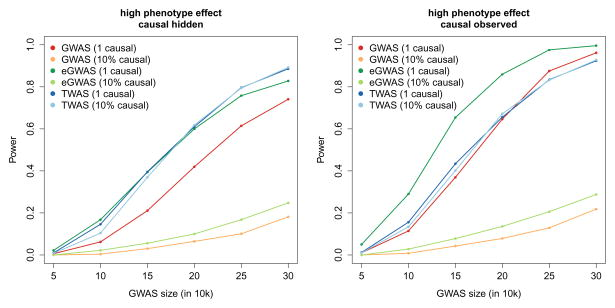
\includegraphics[width=\textwidth]{gusev2016/5-association_power}
	\end{figure}

	\note[item]{Allelic heterogeneity}

\end{frame}

\begin{frame}{Causality models}

	\begin{figure}
		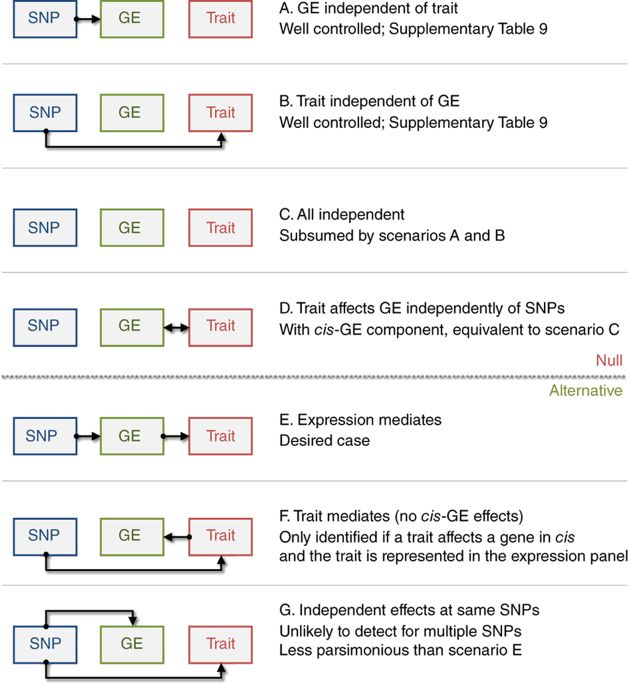
\includegraphics[width=0.5\textwidth]{gusev2016/2-causality_models}
	\end{figure}

\end{frame}

\begin{frame}{Heritability and prediction of gene expression}

	\begin{figure}
		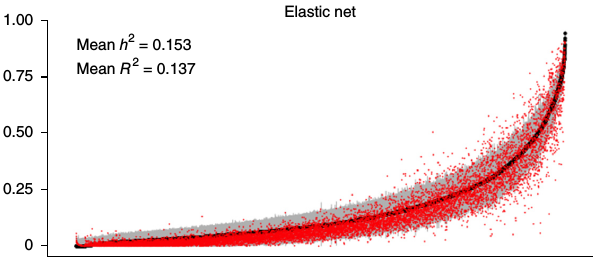
\includegraphics[width=\textwidth]{gamazon2015/3-prediction_r2}
	\end{figure}

\end{frame}

\begin{frame}{Different levels of phenotype}

	\begin{figure}
		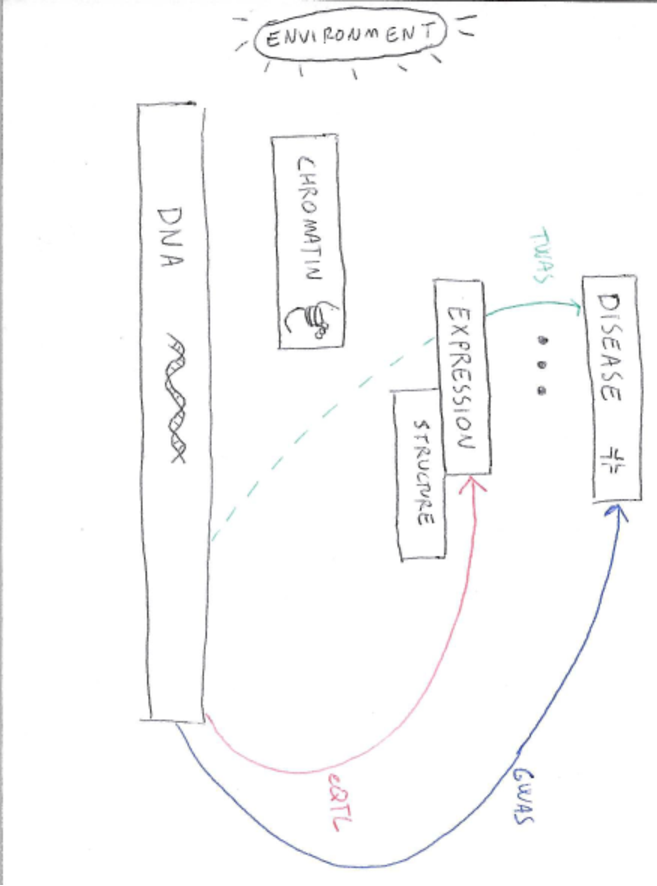
\includegraphics[width=0.9\textwidth]{introduction/summary}
	\end{figure}

\end{frame}

\end{document}

% ### Reference

% Dual screen with notes:

% To display notes on second screen, do the following. First you have to 
% set up the projector: open the display settings and choose "join 
% displays". (mirror just copies the pc monitor on the projector; single 
% display neglects one of the displays.) Set the built-in display as the 
% primary one. You can also set the resolution for each display, e.g. 
% for the PC you can set 16:9 and for the projector 4:3 or whatever is 
% available. This will create two displays, and you can switch from one 
% another moving the mouse cursor to the appropriate site.
% At this point you have to run the presentation, using a tool capable 
% to exploit dual screens. There are several options:
% pympress. On the command line, write pympress, then open the right 
% file. It does not always work, and the presentation in 16:9 does not 
% fit the projector display.
% dspdfviewer. On the command line, write dspdfviewer main.pdf. It will 
% work out of the box.
% pdfpc. On the command line, pdfpc main.pdf --notes=right. It can also 
% work out of the box, without the options. If you use the option 
% --notes, specify the same value you had specified to pgfpages inside 
% the .tex file. It also handles overlays (I still have to investigate 
% this feature). However, in dspdfviewer I can see both the current 
% slide and the notes; besides, the space for the notes is bigger.

% Graphics: figure environment

%\begin{figure}
%	\centering
%	\includegraphics[width=0.8\textwidth, keepaspectratio]{imgname}
%\end{figure}

% Interactive global structure: framezoom

%\framezoom<1><2>[border](5.5cm,0.5cm)(1cm,1cm)
%\begin{figure}
% 	\includegraphics[width=2cm,height=2cm]{imgname}
%\end{figure}
